\section{Ungedämpfte Schwingungen}

\subsection{Schwingungen -- Übersicht}

\paragraph{Freie Schwingung}

Wird ein schwingungsfähiges System aus dem Gleichgewichtszustand gebracht 
und dann sich selbst überlassen, so führt es freie Schwingungen oder Eigenschwingungen aus.


\medskip

\paragraph{Erzwungene / Fremderregte Schwingung}

Wird ein System von aussen durch periodische oder auch nichtperiodische Störungen zum
Schwingen veranlasst, wird von fremderregten Schwingungen gesprochen. 


\medskip

\paragraph{Selbsterregte Schwingung}

Ein schwingungsfähiges System kann unter Umständen einer Energiequelle Energie entziehen
und diese der eigenen Schwingung selbst zuführen, so dass die Schwingung trotz einer
eventuell vorhandenen Dämpfung nicht abklingt. 


\subsection{Freie Schwingungen}

\subsubsection{Terminologie}

\vspace{-0.2cm}
$$ \boxed{  y(t) = A \cdot \sin(\omega \, t + \varphi) } $$
\[
    \dot{y}(t) =  v(t) = A \cdot \omega \cdot \cos(\omega \, t + \varphi) 
    \qquad \qquad \quad
    \ddot{y}(t) = a(t) = - A \cdot \omega^2 \cdot \sin(\omega \, t + \varphi) 
\]
\[
    \boxed{ f = \frac{\omega}{2 \, \pi} }
    \qquad \qquad \qquad \qquad \qquad \qquad
    \boxed{ T = \frac{1}{f} = \frac{2 \, \pi}{\omega} }
\]


\renewcommand{\arraystretch}{1.3}
\begin{ctabular}{clc}
    $y(t)$          & Position zum Zeitpunkt $t$        & $[y(t)] = \meter$                             \\
    $\dot{y}(t)$    & Geschwindigkeit zum Zeitpunkt $t$ & $[\dot{y}(t)] = \frac{\meter}{\second}$       \\ 
    $\ddot{y}(t)$   & Beschleunigung  zum Zeitpunkt $t$ & $[\ddot{y}(t)] = \frac{\meter}{\second^2}$    \\ 
    $A$             & Amplitude                         & $[A] = \meter$                                \\
    $\omega$        & Winkelgeschwindingkeit            & $[\omega] = \frac{\rad}{\second}$             \\
    $\varphi$       & Phase                             & $[\varphi] = \rad$                            \\ 
    $T$             & Periodendauer                     & $[T] = \second$                               \\
    $f$             & Frequenz                          & $[f] = \frac{1}{\second}$
\end{ctabular}
\renewcommand{\arraystretch}{1}


\example{Federpendel}

\begin{minipage}{0.48\columnwidth}
    $$F_{\rm res} = m \cdot a = m \cdot \ddot{x}$$ 
\end{minipage}
\hfill
\begin{minipage}{0.48\columnwidth}
    $$F_{\rm Feder} = -k \cdot x$$
\end{minipage}

$$ \text{Kräftegleichgewicht:} \quad m \cdot \ddot{x} = -k \cdot x $$
\[ 
    \boxed{ \text{DGL: } \ddot{x} = - \omega^2 \cdot x \quad \text{mit } \omega^2 = \frac{k}{m} } 
    \qquad \quad
    \text{Allgemeine Lösung:} \quad  x(t) = A \cdot \sin(\omega \, t + \varphi) 
\]

\begin{ctabular}{clc}
    $m$     & Masse             & $[m] = \meter$                    \\
    $k=c$   & Federkonstante    & $[k] = \frac{\newton}{\meter}$
\end{ctabular}


\subsubsection{Harmonische Schwingung -- Energiebetrachtung}

\vspace{-0.2cm}

\[
    \cbl{x(t) = A \cdot \sin(\omega \, t + \varphi)} 
    \qquad \qquad \qquad
    \cvt{\dot{x}(t) = \omega \cdot A \cdot \cos(\omega \, t + \varphi)}
\]

\vspace{-0.2cm}

\begin{align*}
    E_{\rm tot} &= E_{\rm pot} + E_{\rm kin} = \frac{k \cdot \cbl{x^2} }{2} + \frac{m \cdot \cvt{\dot{x}^2 } }{2}   \\
                &= \frac{k}{2} A^2 \cdot \sin^2(\omega \, t + \varphi) + \frac{m}{2} \omega^2  A^2 \cdot \cos^2(\omega \, t + \varphi) \\
                &= \frac{k A^2}{2} ( \sin^2(\omega \, t + \varphi) + \cos^2(\omega \, t + \varphi) )
\end{align*}

$$ \boxed{ E_{\rm tot} = \frac{k \cdot A^2}{2} } $$


\subsection{Beschreibung einer 1D-Schwingung}

\subsubsection{Zeitbreich}

\begin{minipage}[t]{0.42\columnwidth}
    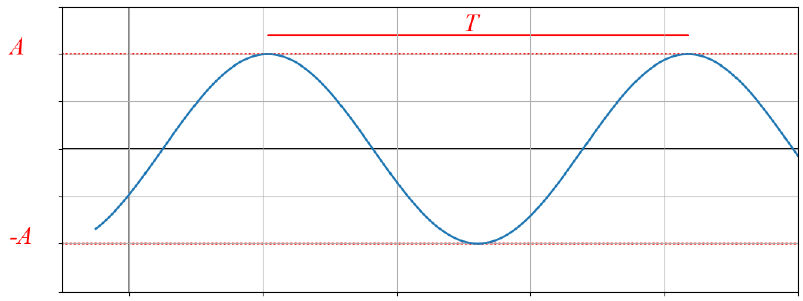
\includegraphics[width=\columnwidth, align=t]{images/zeitbereich.png}
\end{minipage}
\hfill
\begin{minipage}[t]{0.52\columnwidth}
    Auslenkung in Abhängigkeit der Zeit \\
    Beispiel: Oszilloskop 
    $$ x(t) = A \cdot \sin(\omega \, t + \varphi) $$
\end{minipage}


\subsubsection{Zeigerdarstellung}

\begin{minipage}[c]{0.4\columnwidth}
    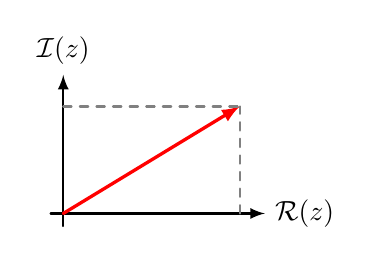
\begin{tikzpicture}
    [>=latex, 
    line cap=round,
    line join=round,
    scale=0.8]

    \draw[->, thick] (-0.2, 0  ) -- (3.2, 0 ) node[right] {$\mathcal{R}(z)$};
    \draw[->, thick] (0,   -0.2) -- (0,  2.2) node[above] {$\mathcal{I}(z)$};
        
    \draw[->, very thick, red] (0, 0) -- (2.8, 1.7);

    % Hilfslinien
    \draw[dashed, thick, gray] (2.8, 0) -- (2.8, 1.7);
    \draw[dashed, thick, gray] (0, 1.7) -- (2.8, 1.7);
\end{tikzpicture}
\end{minipage}
\hfill
\begin{minipage}[c]{0.56\columnwidth}
    Auslenkung als Zeiger (komplexe Zahl), der um den Ursprung rotiert 
    $$ z(t) = \underbrace{ x(t) }_{\substack{\mathcal{R}(z)}} + i \, \underbrace{ y(t) }_{\substack{ \mathcal{I}(z)}} $$
\end{minipage}


\subsubsection{Phasenraum}

\begin{minipage}[c]{0.4\columnwidth}
    
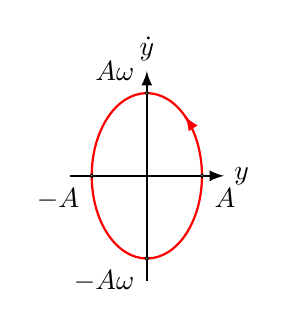
\begin{tikzpicture}[>=latex, scale=0.7]

  % Ellipse
  \draw[thick, red] (0,0) ellipse (1 and 1.5);

  % Achsen
  \draw[->, thick] (-1.4,0) -- (1.4,0) node[right] {$y$};
  \draw[->, thick] (0,-1.9) -- (0,1.9) node[above] {$\dot{y}$};

  % Beschriftungen
  \node at (1,0) [below right=1pt] {$A$};
  \node at (-1,0) [below left=1pt] {$-A$};
  \node at (0,1.5) [above left=1pt] {$A\omega$};
  \node at (0,-1.5) [below left=1pt] {$-A\omega$};

  % Punkte auf Ellipse
  \filldraw[white, draw=black] (1,0) circle (0.03);
  \filldraw[white, draw=black] (-1,0) circle (0.03);
  \filldraw[white, draw=black] (0,1.5) circle (0.03);
  \filldraw[white, draw=black] (0,-1.5) circle (0.03);

  % Pfeil auf der Ellipse
  \draw[->, red, thick, domain=45:46] plot ({cos(\x)}, {1.5*sin(\x)});
\end{tikzpicture}
\end{minipage}
\hfill
\begin{minipage}[c]{0.54\columnwidth}
    Darstellung der Position $y$ und der Ableitung (Geschwindigkeit)
\end{minipage}


\subsection{Pendel}

\subsubsection{Fadenpendel}

\begin{minipage}{0.27\columnwidth}
    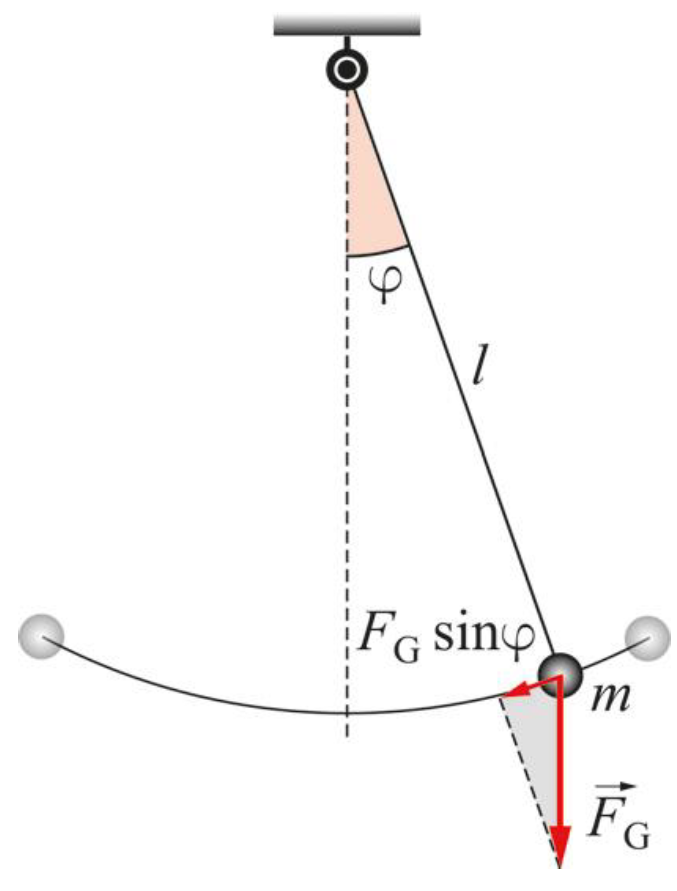
\includegraphics[width=\columnwidth]{images/fadenpendel.png}
\end{minipage}
\hfill
\begin{minipage}{0.7\columnwidth}
    $$ F_R = F_G \cdot \sin(\varphi) = m \cdot g \cdot \sin(\varphi) \approx m \cdot g \cdot \varphi $$
    $$ x = \varphi \cdot l \quad \rightarrow \quad \varphi = \frac{x}{l} $$
    $$ \Rightarrow F_G = m \cdot g \cdot \frac{x}{l} $$
   
    $$ \text{Kräftegleichgewicht:} \quad  F = m \cdot \ddot{x} = - m \cdot g \, \frac{x}{l} $$
    $$ \boxed{ \text{DGL:} \quad  \ddot{x} = - \omega^2 \cdot x \quad \text{mit } \omega^2 = \frac{g}{l} } $$
\end{minipage}


\subsubsection{Drehpendel}

\begin{minipage}[t]{0.36\columnwidth}
    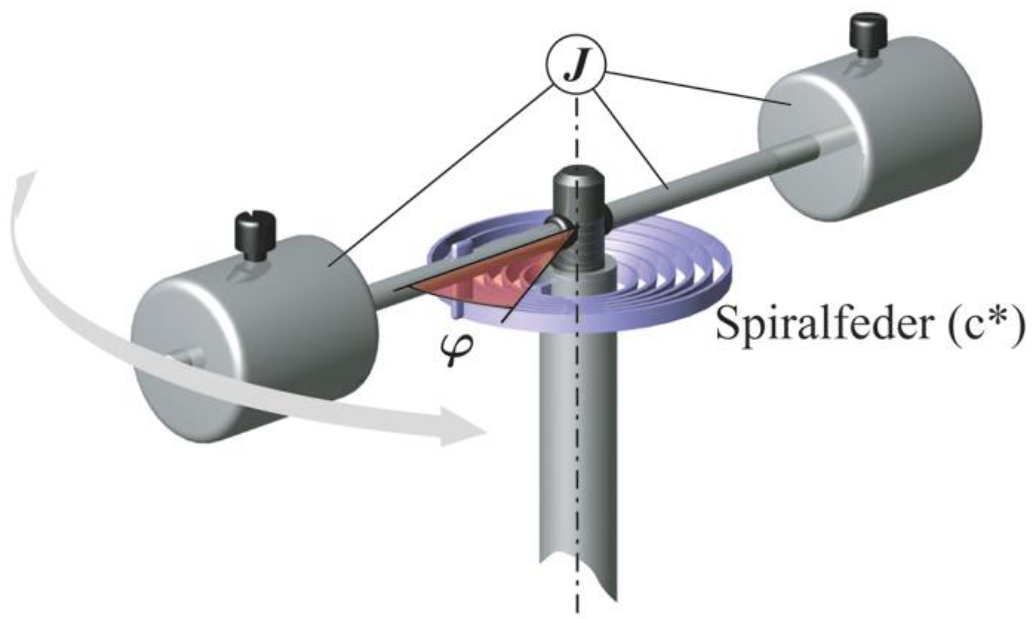
\includegraphics[width=\columnwidth, align=t]{images/drehpendel.png}
\end{minipage}
\hfill
\begin{minipage}[t]{0.6\columnwidth}
    \paragraph{Analogie ohne Rotation}

    \begin{minipage}[c]{0.58\columnwidth}
        $F = - k \cdot x$ \\
        $ M = - c^* \, \varphi$ 
    \end{minipage}
    \hfill
    \begin{minipage}[c]{0.4\columnwidth}
         $F = m \cdot a = m \cdot \ddot{x}$ \\
         $M = J \cdot \ddot{\varphi} $ 
    \end{minipage}

    $$ \text{Gleichgewicht:} \quad  J \cdot \ddot{\varphi} = - c^* \, \varphi $$
    $$ \boxed{ \text{DGL: } \ddot{\varphi} = - \omega^2 \cdot\varphi \quad \text{mit } \omega^2 = \frac{c^*}{J} }$$
\end{minipage}

\medskip

$\varphi$ folgt der gleichen DGL wie $x$ im Fall des Federpendels und hat die Lösung:
$$ \varphi(t) = \varphi_0 \cdot \sin(\omega \, t + \delta) $$

\renewcommand{\arraystretch}{1.3}
\begin{ctabular}{clc}
    $J$     & Trägheitsmoment   & $[J] = \kilogram \cdot \meter\squared$    \\
    $c^*$   & Winkelrichtgrösse & $[c^*] = \mathrm{\frac{N \, m}{rad}}$
\end{ctabular}
\renewcommand{\arraystretch}{1}



\subsubsection{Torisonpendel}
\begin{minipage}[t]{0.12\columnwidth}
    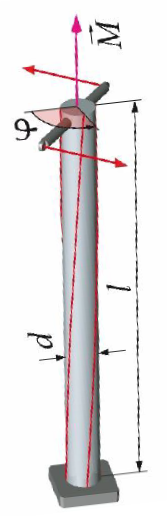
\includegraphics[width=\columnwidth, align=t]{images/torsionspendel.png}
\end{minipage}
\hfill
\begin{minipage}[t]{0.8\columnwidth}
    Variante des Drehpendels mit der Winkelrichtgrösse

    $$ \boxed{ c^* = \frac{\pi r^4 G}{2l} } $$  

    \begin{ctabular}{ll}
        $G$                 & Torsionsmodul \\
        $l$                 & Länge         \\
        $r = \frac{d}{2}$   & Radius
    \end{ctabular}
\end{minipage}


\subsubsection{Physikalisches Pendel}

\begin{minipage}{0.3\columnwidth}
    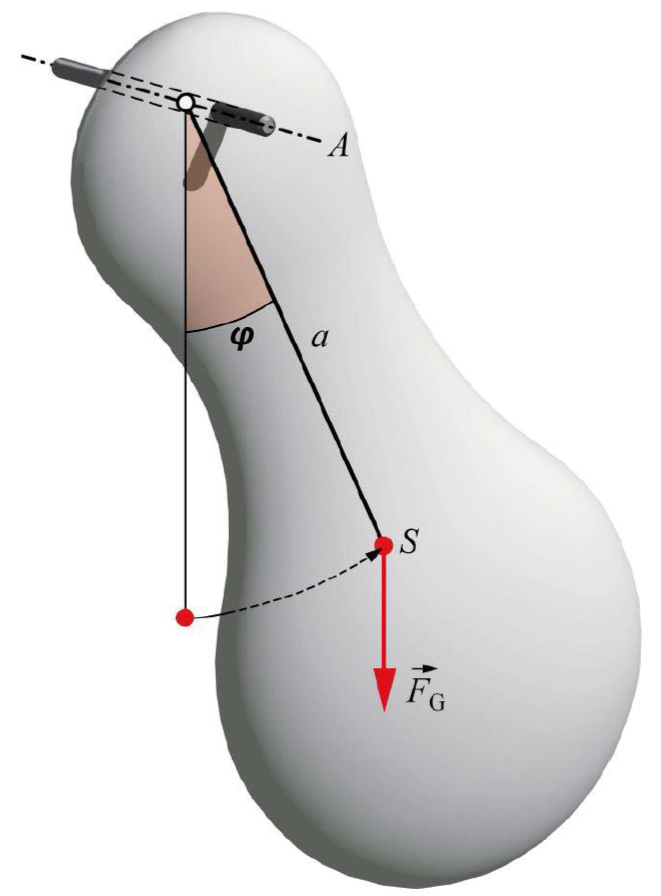
\includegraphics[width=\columnwidth]{images/physikalisches_pendel.png}
\end{minipage}
\hfill
\begin{minipage}{0.68\columnwidth}
    \vspace{-0.2cm}
    $$ M = - a \cdot \sin(\varphi) \cdot F_G = -a \cdot m \cdot g \cdot  \sin(\varphi) $$

    \begin{tabular}{ll}
        Bewegungsgleichung: & $M = J_A \cdot \ddot{\varphi}$                                            \\
        Gleichgewicht:      & $-a \cdot m \cdot g \cdot  \sin(\varphi) =  J_A \cdot \ddot{\varphi}$     \\
        Kleine Winkel:      & $-a \cdot m \cdot g \cdot \varphi =  J_A \cdot \ddot{\varphi}$            \\
    \end{tabular}

    $$ \boxed{ \text{DGL: } \ddot{\varphi} = -\omega^2 \, \varphi  \quad \text{mit } \omega^2 =  \frac{g}{L^*} = \frac{g \cdot a \cdot m}{J_A}  }$$
    $$ \boxed{L^* = \frac{J_A}{a \cdot m}} \qquad \boxed{J_A = J_s + m \cdot a^2 } $$  

    \medskip
    $\varphi$ folgt der gleichen DGL wie $x$ im Fall des Federpendels
\end{minipage}

\medskip

\paragraph{Physikalisches Pendel mit mehreren Massen}

\vspace{-0.2cm}

\begin{minipage}[c]{0.46\columnwidth}
    $$ \boxed{  T = \frac{2 \, \pi}{\omega} = 2 \, \pi \sqrt{\frac{J_{A1} + J_{A2}}{(a_1 \cdot m_1 + a_2 \cdot m_2) \cdot g}} } $$
\end{minipage}
\hfill
\begin{minipage}[c]{0.52\columnwidth}
    \textbf{ \textrightarrow\ $\bm{J}$-Tabelle im Anhang Abschnitt \ref{Massenträgheitsmomente}}
\end{minipage}

\begin{ctabular}{clc}
    $S$     & Schwerpunkt des Körpers           &                                           \\
    $J_s$   & Trägheitsmoment bzgl. $S$         & $[J_S] = \kilogram \cdot \meter\squared$  \\
    $a$     & Abstand Schwerpunkt -- Drehpunkt  & $[a] = \meter$                            \\
    $L^*$   & Reduzierte Länge                  & $[L^*] = \meter$                          \\
    $J_A$   & Trägheitsmoment um Aufhängepunkt  & $[J_A] = \kilogram \cdot \meter\squared$ 
\end{ctabular}


\subsection{Perkussionszentrum}

\textbf{Frage:} Wie weit vom Drehpunkt $A$ muss ein Impuls auf einen Körper ausgeübt werden, damit keine Kraft auf die Achse ausgeübt wird?

\smallskip

\textbf{Antwort:} Auf Höhe der \textbf{reduzierten Länge} $L^* = \frac{J_A}{a \cdot m}$

\begin{center}
    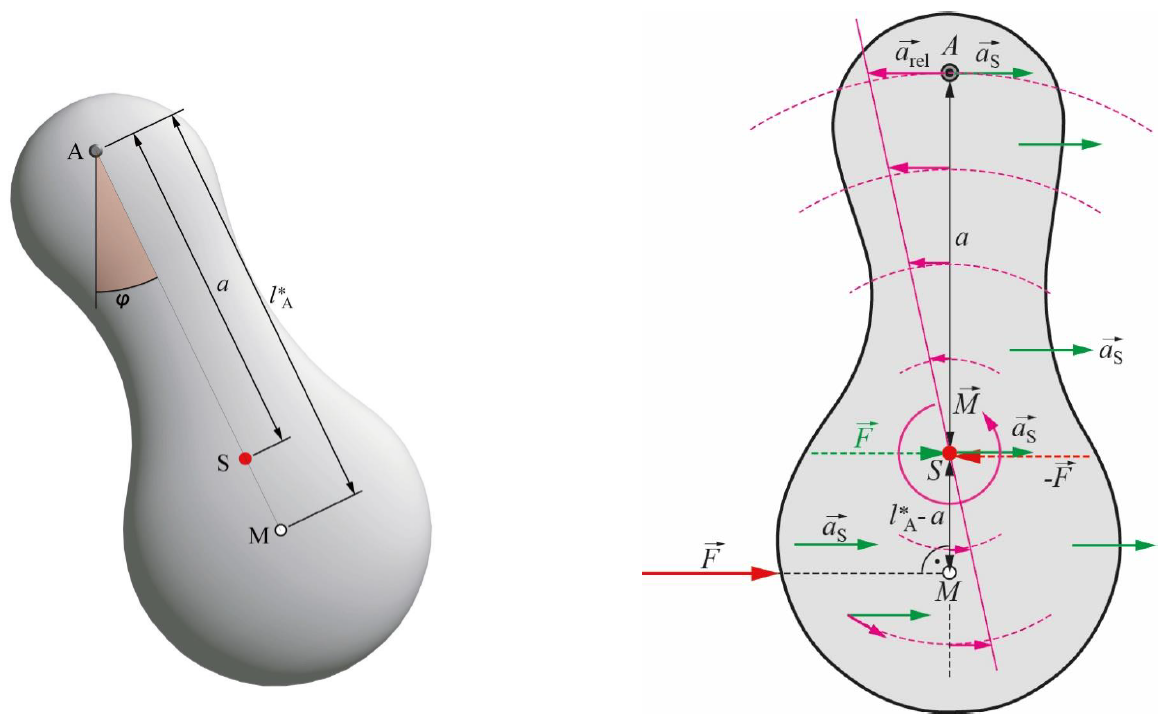
\includegraphics[width=0.7\columnwidth]{images/perkussionszentrum.png}
\end{center}



\subsection{Periodische Schwingung}

\begin{minipage}{0.4\columnwidth}
    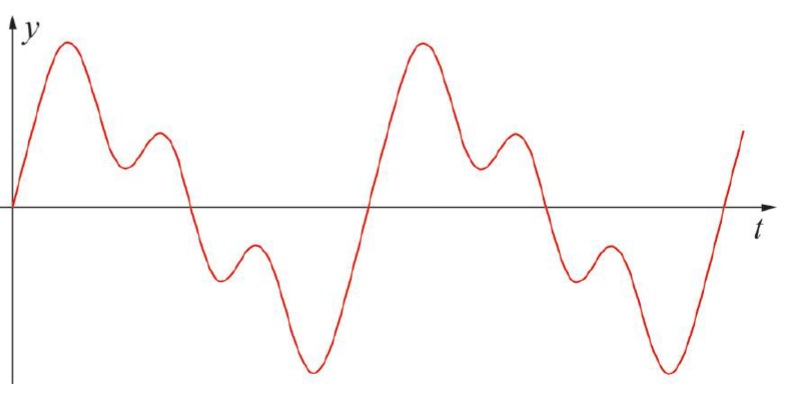
\includegraphics[width=\columnwidth]{images/periodische_schwingung.png}
\end{minipage}
\hfill
\begin{minipage}{0.56\columnwidth}
    Muster wiederholt sich mit Periode $T$
    $$ \boxed{ f(t) = f(t - T ) }$$
\end{minipage}

\smallskip

Periodische Schwingungen können im \textbf{Frequenzbereich} in eine \textbf{Grundschwingung} und \textbf{Oberschwingungen} \textbf{(Harmonische)} zerlegt werden. 

\begin{minipage}[c]{0.48\columnwidth}
    $$ \boxed{ f(t) = A_0 + \sum\limits_{n=1}^{\infty}  A_n \, \sin(n \cdot \omega + \varphi_n) } $$
\end{minipage}
\hfill
\begin{minipage}[c]{0.48\columnwidth}
    \renewcommand{\arraystretch}{1.3}
    \begin{tabular}{ll}
        $\omega_0 = \frac{2 \, \pi}{T}$     & Grundschwingung   \\
        $\omega_n = n \cdot \omega_0$       & $n$-te Harmonische
    \end{tabular}
    \renewcommand{\arraystretch}{1}
\end{minipage}





\subsubsection{Fourier-Analyse}

\vspace{-0.2cm}

$$ \boxed{ f(t) = A_0 +  \sum\limits_{n=1}^{\infty}  A_n \cdot \cos  \left(\frac{ 2 \, \pi \, n}{T} t \right) + \sum\limits_{n=1}^{\infty}  B_n \cdot \sin \left( \frac{ 2 \, \pi \, n}{T} t \right)  } $$


\begin{minipage}{0.48\columnwidth}
    \centering
    $ A_n = \frac{2}{T} \int\limits_{-T/2}^{T/2} f(t) \, \cos \Big(\frac{ 2 \, \pi \, n \, t}{T}  \Big)  \, \dd t $
\end{minipage}
\hfill
\begin{minipage}{0.48\columnwidth}
    \centering
    $A_0 = \frac{1}{T} \int\limits_{-T/2}^{T/2} f(t) \, \dd t $
\end{minipage}

\medskip

\begin{minipage}{0.48\columnwidth}
    \centering
    $ B_n = \frac{2}{T} \int\limits_{-T/2}^{T/2} f(t) \, \sin \Big(\frac{ 2 \, \pi \, n \, t}{T}  \Big)  \, \dd t $
\end{minipage}
\hfill\null%



\subsection{Signalmodulationen}

\begin{minipage}[t]{0.43\columnwidth}
    $$ \boxed{ x(t) = A \sin ( \omega t + \varphi)} $$ 

    \paragraph{ Amplitudenmodulation (AM)}
    Veränderung von $A$ 

    \medskip

    \paragraph{Frequenzmodulation (FM)}
    Veränderung von $\omega$
\end{minipage}
\hfill
\begin{minipage}[t]{0.55\columnwidth}
    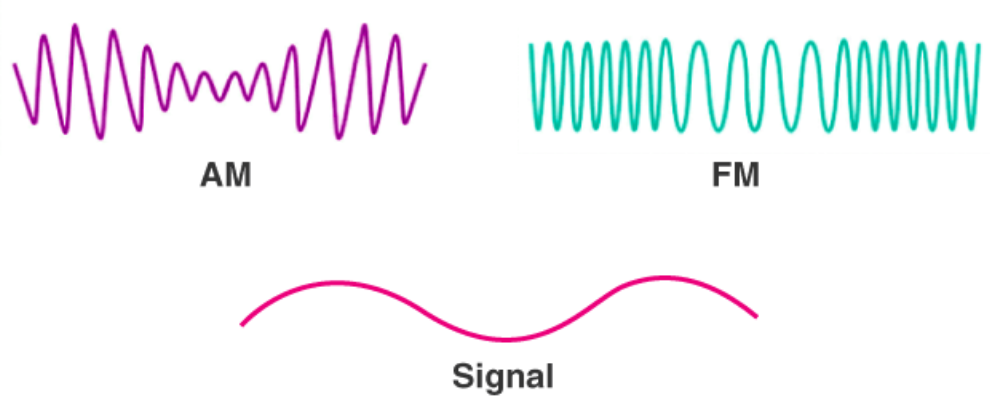
\includegraphics[width=\columnwidth, align=t]{images/AM_FM.png}
\end{minipage}


